% !TeX root = ../thuthesis-example.tex

\chapter{引言}

触摸交互是自然人机交互的重要组成部分,是人主动控制手指触摸交互表面,通过点击、长按、滑动等手势向计算机输入信息的方式。触摸屏作为触摸交互的主要载体已问世数十年,然而,触摸交互在普适性、响应性和意图性上仍然存在很大的改进空间:为提供最佳用户体验,触摸交互应摆脱有源交互表面的束缚,拓展至无源的桌面、墙面上;触摸交互的端到端延迟应控制在20毫秒以内,以免人察觉到延迟;触摸交互的防误触能力应落实到人的意图层面,任何不表达输入意图的触摸都应被过滤。在此背景下,本文提出触摸运动模型,揭示触摸前后极短时间内手指的运动规律,即手指位移、速度和加速度的时空运动特征,对增强触摸交互的普适性、响应性和意图性具有指导意义。本章首先介绍触摸交互的重要性和优化空间,随后通过文献综述总结现有触摸交互技术及其不足,接下来简述触摸运动模型及其研究内容,最后介绍论文的组织结构。

\section{选题背景及意义}

\subsection{触摸交互的重要性}

触摸交互是当前最重要的人机交互方式之一。2021年,手机、平板电脑等触摸屏设备的全球出货量达到15.1亿台,而笔记本、台式机等基于键鼠交互的设备的全球出货量为3.6亿台\cite{alsop2020shipment},其规模仅为触摸屏设备的23.8\%。相比于键鼠交互,触摸交互具有便捷、易学、自然等优势,使其适用于包括老人、儿童在内的更广泛用户群体。

\begin{figure}
	\centering
	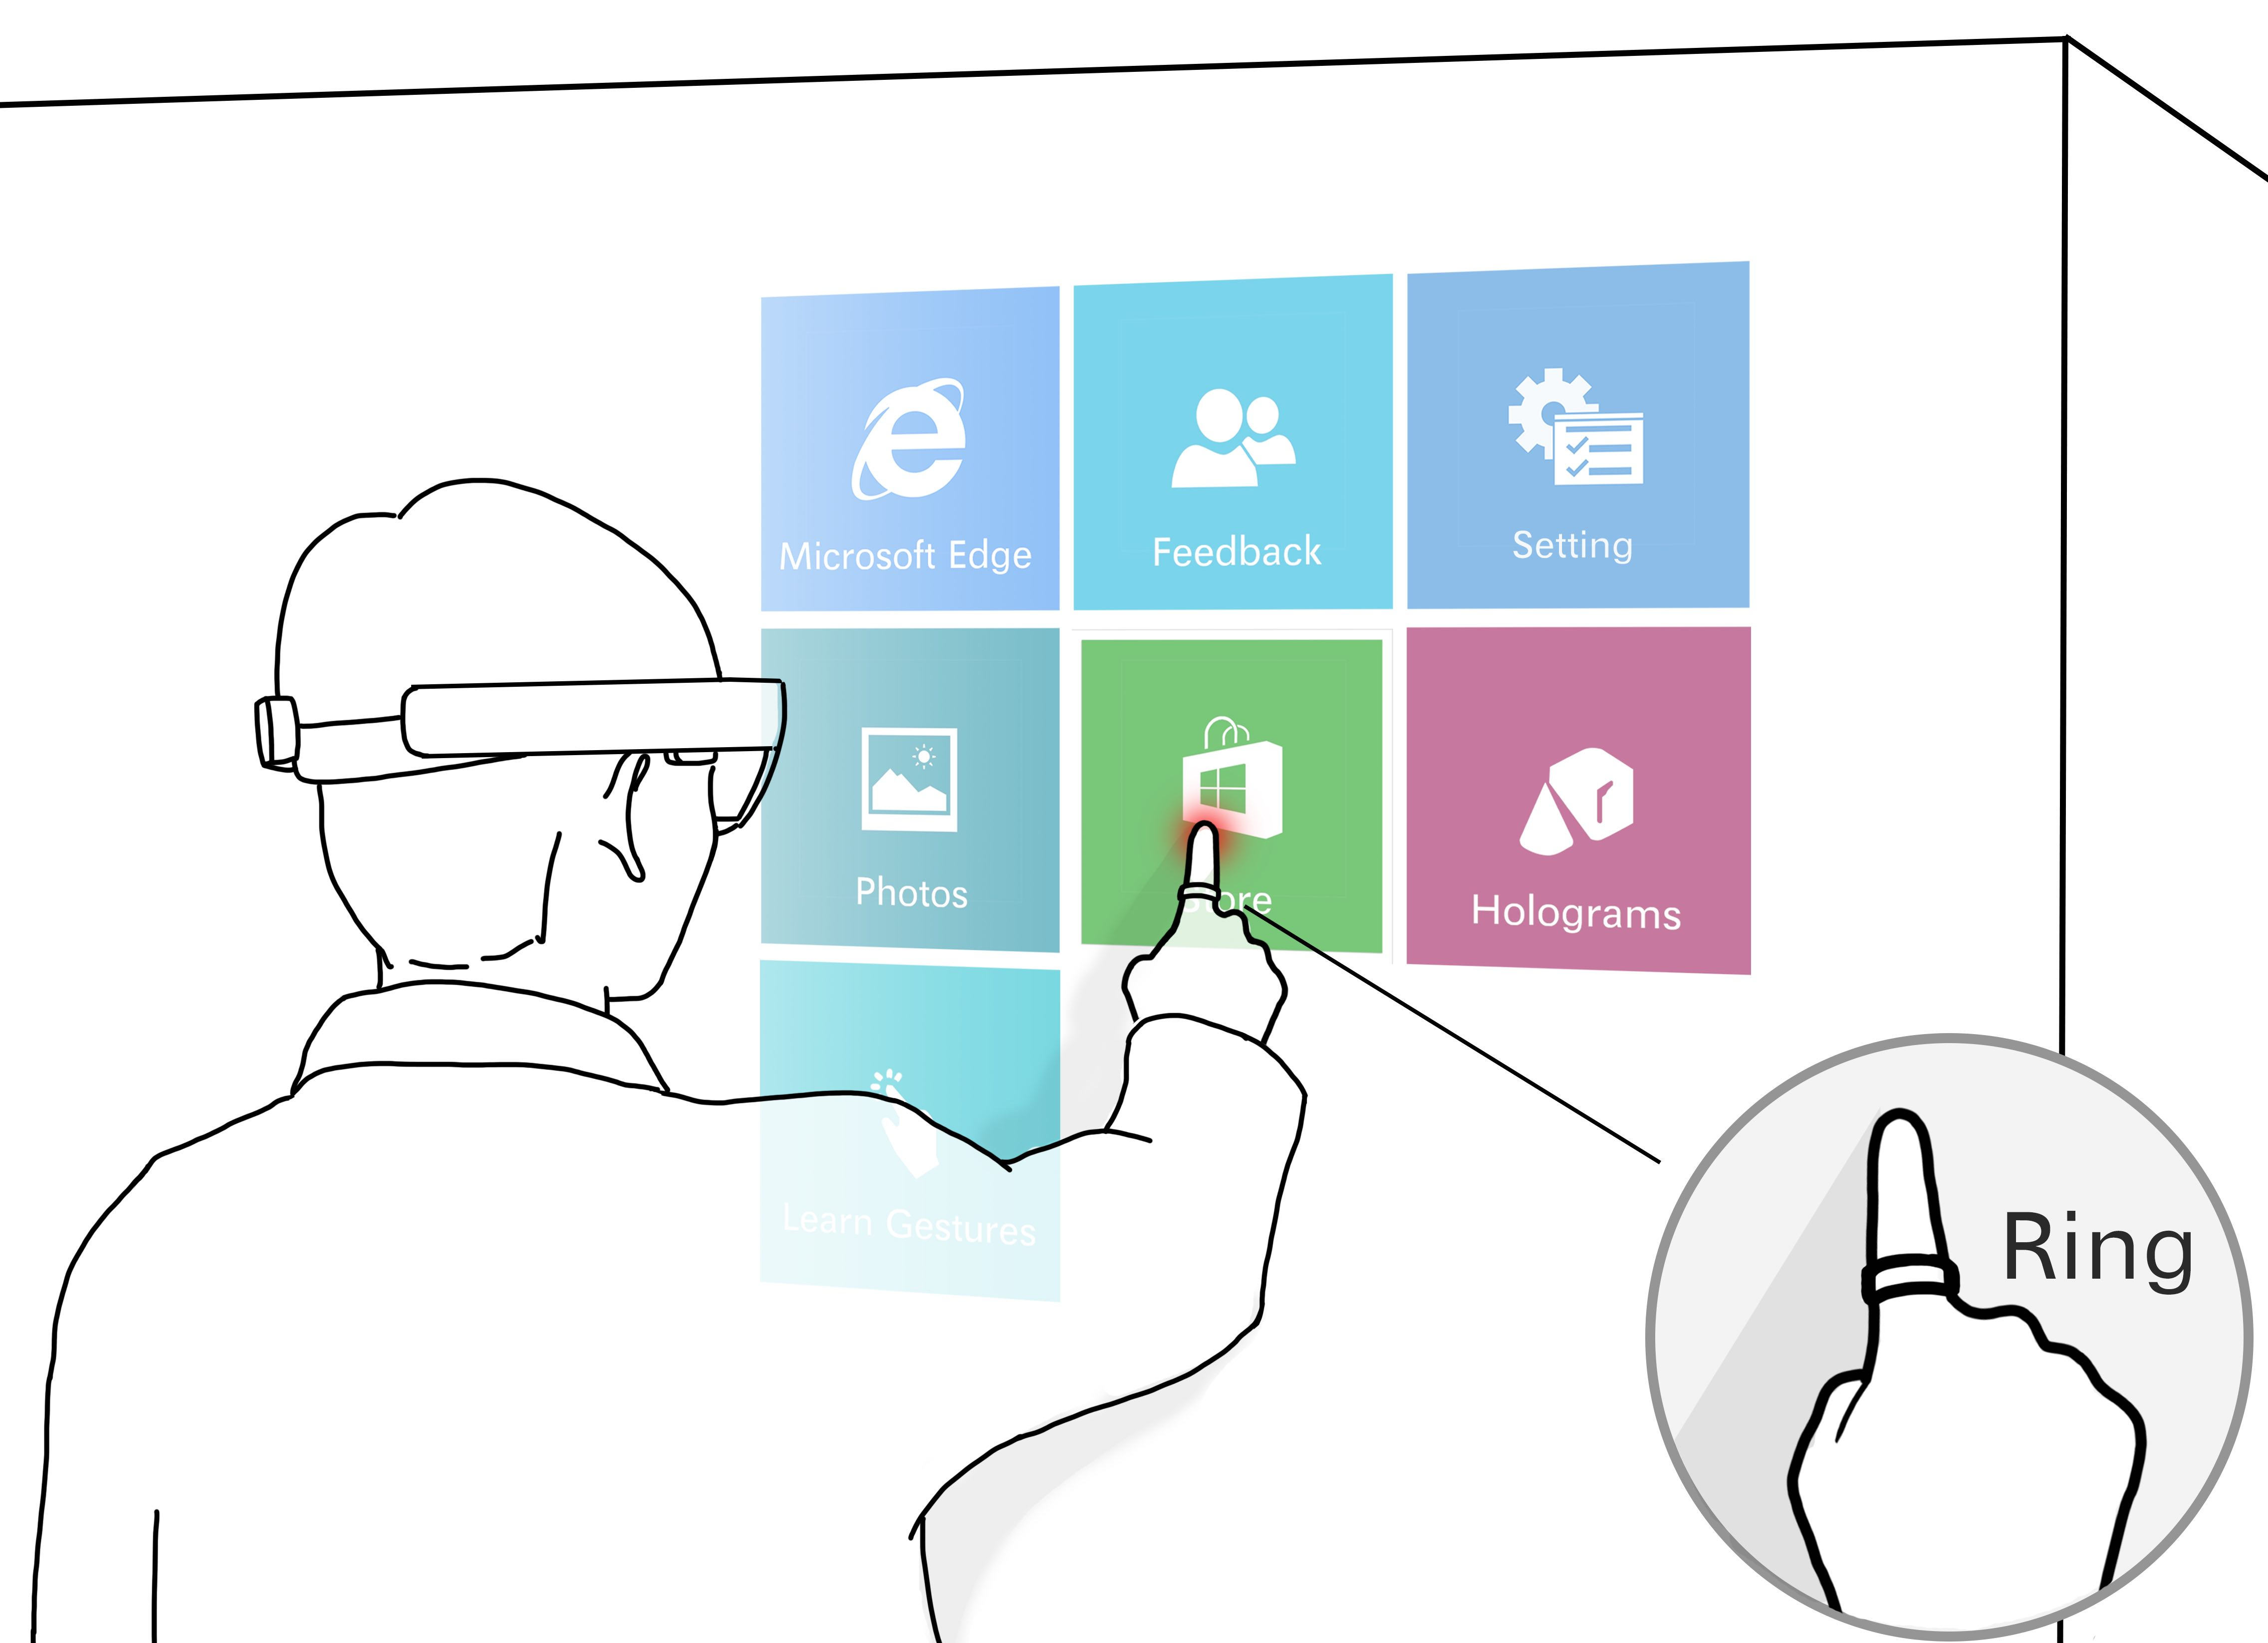
\includegraphics[width=0.8\linewidth]{MR_touch_envision.jpg}
	\caption*{在未来的可穿戴场景下,人应能在普通的表面如桌面、墙面上通过触摸交互向计算机输入信息。}
	\caption{无源表面触摸交互的构想}
	\label{fig:MR_touch_envision}
\end{figure}

在未来,触摸交互仍是人机交互的重要研究课题。头戴式混合现实设备(简称MR头盔,例如微软的Hololens2\cite{hololens2})很可能取代手机成为下一代智能终端。MR头盔利用深度摄像头扫描物理环境,将虚拟元素叠加渲染在物理实体之上。如图\ref{fig:MR_touch_envision}所示,MR头盔中一种有前景的交互方式是将虚拟的用户界面渲染在无源表面上,支持用户通过触摸与用户界面交互\cite{gu2019accurate}。其中,\textbf{无源表面}指的是无(电)能源的表面,在本文中,无源表面特指生活中常见的非数字化表面,如桌子表面、墙面、人的手掌等等。在此设想下,触摸交互将摆脱有源触摸屏的束缚,让人获得在无源表面上触摸输入的能力。与目前MR头盔中流行的空中手势交互相比,触摸交互具有更高的效率和精度、更佳的主观用户体验\cite{jakobsen2015should}。然而,目前无源表面的触摸交互技术仍未成熟,需要进一步研究。

\subsection{触摸交互的改进空间}

尽管触摸屏已经问世数十年,但是触摸交互技术仍然在普适性、响应性和意图性三方面存在很大的改进空间。人的交互体验是人机交互的重要研究课题,因此,本小节以最佳用户体验为导向,讨论触摸交互技术的改进空间:

\textbf{(1)普适性}:普适计算是一个强调和环境融为一体的计算概念,主张计算设备朝小型化、可穿戴的方向发展,直至消失在人们的视线当中,人们能在任何时间、地点,以任何方式与与数字世界交互。在人机交互往普适计算发展的过程中,触摸屏等有源输入设备可能是第一批消失的,在此背景下,如何支持无源表面(如桌面、墙面、手掌)的触摸交互,是值得研究的课题。

\textbf{(2)响应性}:响应性包括触摸检测的准确性和延迟两方面。触摸检测的准确性是触摸交互的基础,是人能否顺利完成交互任务的关键;人对触摸交互延迟的感官需求极高,能察觉到低至24毫秒的延迟\cite{jota2013fast},高于100毫秒的延迟会让用户感到极度厌烦\cite{miller1968response},且影响交互效率\cite{jota2013fast, ng2012designing}。因此,若要提供最佳的用户体验,必须将触摸检测准确率提高至99\%以上,延迟降低至20毫秒以内。

\textbf{(3)意图性}:自然触摸交互中人的有意触摸和无意触碰混杂,给防误触技术带来困难。最佳的防误触技术应从用户意图的层面出发,将误触定义为任何不表达交互意图的触摸,过滤所有不表达交互意图的触摸,只对表达交互意图的触摸做出相应。然而,目前的触摸屏只能过滤轻敲、边缘误触等特殊的误触情况,防误触能力仍然需要改进。

电容触摸屏作为目前触摸交互的主要载体,在普适性、响应性和意图性上都远未达到优化目标,存在较大的改进空间。需要补充的是,在触摸交互技术的发展过程中,还曾存在\textbf{精准性}问题,即触摸2D位置的识别精度问题。然而,相比于鼠标交互,触摸交互是不精准的——人用手指能点中的最小目标直径为4.3毫米(点中概率为95\%)。造成触摸交互不精准的主要原因是胖手指问题\cite{yi2017too},而非触摸交互技术不够精准,这使得继续优化触摸交互精准性对人机交互体验的意义不大。因此,触摸交互的精准性不在本文的讨论范围内。

\subsection{为什么要建立触摸运动模型?}

上一小节提到,触摸交互技术发展到今天,仍存在很大的改进空间。在此背景下,建立触摸运动模型能为触摸交互技术在普适性、响应性和意图性上的优化提供计算理论基础。其中,“运动”一词是本模型能够指导触摸交互技术的关键所在:

(1)在普适性方面,触摸交互技术朝着无源表面触摸的方向发展。文献调研发现,近二十年来共有29篇关于无源表面触摸交互的高水平论文,它们全部依赖位移、速度和加速度等运动信号。其中,15篇论文利用基于视觉的位移传感\cite{harrison2011omnitouch, xiao2018mrtouch, paradiso2000sensor, agarwal2007high, chang2005real, letessier2004visual, sugita2008touch, grudin2001integrating, saba2012dante, xiao2016direct, benko2012miragetable, wilson2010combining, newcombe2011kinectfusion, mistry2011mouseless, xiao2013worldkit},3篇论文利用基于磁力的位移传感\cite{chan2013fingerpad, chen2013utrack, parizi2019auraring},8篇论文利用到基于惯性传感器的加速度传感\cite{gu2019accurate, shi2020ready, gu2020qwertyring, meier2021tapld, lam2002mids, oh2017anywheretouch, niikura2014anywhere, liu2020keep},3篇论文利用到基于麦克风的震动传感\cite{chan2013fingerpad, chen2013utrack, parizi2019auraring}。以上观察说明,触摸交互技术若要摆脱触摸屏的束缚,触摸运动的规律是绕不开的话题。然而,上述论文始终缺少一个底层的模型作为计算理论基础。

\begin{figure}
	\centering
	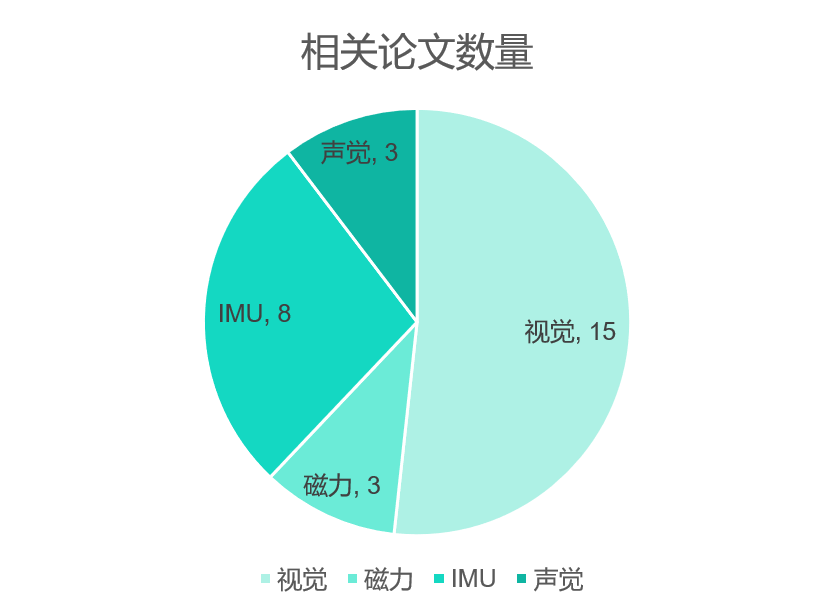
\includegraphics[width=0.6\linewidth]{anywhere_touch_related_work.png}
	\caption*{近二十年29篇关于无源表面触摸交互的论文全部依赖运动信号。其中,视觉和磁力方法代表位移传感,IMU(惯性传感单元)和麦克风代表加速度和震动传感。}
	\caption{无源表面触摸交互的相关论文}
	\label{fig:anywhere_touch_related_work}
\end{figure}

(2)在响应性方面,只有建立起触摸运动模型,触摸检测的准确率和延迟优化才能有理可依。本文的后续分析表明,触摸交互的准确性和延迟优化并非独立的优化问题,而是此消彼长的关系:当一个触摸检测系统允许有更长的识别延迟时,它能用于检测触摸的信息就更丰富,准确率的上限就越高;但相应地,过长的识别延迟会直接影响到人的触摸交互体验。因此,触摸检测的准确性和延迟优化是需要权衡的问题,而触摸运动模型可以在两者的动态平衡中找到最有益于交互体验的解。

(3)在意图性方面,运动信号是最能表征人的触摸意图的信号之一。人在组织一次触摸时,其心理是对手指的运动过程做出规划,并向运动系统发出指令。本文的后续分析表明,基于最优控制理论的触摸运动模型合理地描述了人的触摸心理,其拟合参数也能作为触摸有意性的判断依据。

综上所述,触摸运动模型能刻画人的触摸运动规律,剖析人的触摸心理,从而指导触摸交互技术在普适性、响应性和意图性上的优化。

% 基于视觉的位移传感\cite{harrison2011omnitouch, xiao2018mrtouch, paradiso2000sensor, agarwal2007high, chang2005real, letessier2004visual, sugita2008touch, grudin2001integrating, saba2012dante, xiao2016direct, benko2012miragetable, wilson2010combining, newcombe2011kinectfusion, mistry2011mouseless, xiao2013worldkit}
% 基于磁力的位移传感\cite{chan2013fingerpad, chen2013utrack, parizi2019auraring}
% 基于惯性传感器的加速度传感\cite{gu2019accurate, shi2020ready, gu2020qwertyring, meier2021tapld, lam2002mids, oh2017anywheretouch, niikura2014anywhere, liu2020keep}
% 基于麦克风的震动传感\cite{gong2020acustico, mujibiya2013sound, nakatani2011wearable}

\section{研究现状}

\subsection{触摸交互技术}

触摸交互是手机、平板电脑等手持智能终端上最常用的人机交互方式。大部分触摸交互设备依赖有源的触摸屏技术,需要在交互表面上安装传感器,按技术类型可分为电阻式\cite{downs2005using, hecht2009carbon}、电容式\cite{lee1985multi, wang2009empirical}、光学\cite{han2005low, matsushita1997holowall, wilson2004touchlight}和声学\cite{paradiso2002passive, xiao2014toffee}触摸屏。电容式触摸屏是触摸交互的主要载体,其工作原理是利用低电压交流电场识别人手指与屏幕接触形成的耦合电容。然而,以上触摸屏感知技术要求在所有交互表面上安装传感单元,不可能在可接受的成本内支持普适计算中所展望的随时随地、随心所欲的触摸交互模态,因此,触摸屏交互技术面临普适性不强的问题。为提高触摸交互的普适性,部分研究者致力于将触摸交互从触摸屏的束缚中解放出来,实现无源表面上的触摸交互技术。

%\textbf{无源表面}指的是无(电)能源的交互表面,在本文中,无源表面特指生活中常见的非数字化表面,如桌子表面、墙面、人的手掌等等。

基于摄像头视觉的触摸交互技术是支撑无源表面上触摸交互的方法之一。视觉触摸交互技术可以将摄像头部署在有源触摸屏上\cite{han2005low, matsushita1997holowall,wilson2004touchlight},也可以将摄像头部署在场景空间中,或使用可穿戴的摄像头\cite{harrison2011omnitouch, xiao2018mrtouch},从而支持无源表面触摸交互。相关文献中已经提出了几种用于无源表面触摸检测的视觉方案,包括激光雷达\cite{paradiso2000sensor}、RGB摄像头\cite{agarwal2007high, chang2005real, letessier2004visual, sugita2008touch}、红外摄像头\cite{grudin2001integrating}和热成像摄像头\cite{saba2012dante}等方案。近年来,深度摄像头变得越来越廉价,这引起了研究者们对基于深度摄像头的触摸交互技术的广泛研究,研究内容主要包括交互设计\cite{agarwal2007high, xiao2016direct, xiao2018mrtouch}和精准性问题\cite{xiao2018mrtouch, benko2012miragetable, harrison2011omnitouch, wilson2010combining}。然而,目前的视觉触摸交互技术存在响应性不高的问题,甚至难以准确判断手指是否接触了交互表面\cite{xiao2016direct, xiao2018mrtouch}。已知文献中的视觉触摸交互技术都使用阈值方法传感触摸事件\cite{agarwal2007high, wilson2010combining, harrison2011omnitouch, newcombe2011kinectfusion, xiao2016direct, xiao2018mrtouch}。例如,在代表性工作MRTouch\cite{xiao2018mrtouch}中,研究者利用Hololens混合现实头盔的前置摄像头判断触摸事件的算法流程是:当手指指尖和交互表面之间的距离降至10毫米以内,汇报触摸事件发生;在手指接触交互表面以后,若手指远离交互表面,距离超过了15毫米,则汇报触摸事件结束。MRTouch作为混合现实头盔上最高水平的无源表面触摸交互技术,其未识别率为3.5\%,误触率高达19.0\%,端到端延迟高达180毫秒,这说明视觉触摸交互技术仍需改进。造成上述问题的原因有两点:首先,摄像头对手指和交互表面位置的识别存在误差,特别是对缺少视觉特征点的纯色表面,识别精度更低;其次,从摄像头的位置看去,手指与交互表面的接触位置通常被遮挡,特别是在最有应用前景的混合现实头盔情景下,更是一定会被遮挡。

基于震动的触摸交互技术是支撑无源表面触摸交互的另一种方法,其工作原理是利用惯性传感器或麦克风感知触摸产生的震动和声音,既可以将传感器部署在有源触摸屏上\cite{heo2011forcetap, iwasaki2009expressive, kane2009bonfire, paradiso2002passive, xiao2014toffee},也可以将传感器部署在人的手指\cite{gu2019accurate, shi2020ready, gu2020qwertyring}或手腕\cite{meier2021tapld}上,从而支持无源表面触摸交互。过去,大部分相关工作致力于提高触摸交互的精准性,即提高对手指位置的追踪精度\cite{lam2002mids, oh2017anywheretouch},还有的工作致力于识别用户用哪跟手指进行的触摸\cite{masson2017whichfingers},或者识别交互表面的材质\cite{stearns2018touchcam}。然而,较早前工作忽视了触摸交互的响应性问题,仅利用阈值方法来识别触摸事件的发生\cite{lam2002mids, oh2017anywheretouch, niikura2014anywhere},准确率不超过89.8\%,端到端延迟不低于50毫秒。直到本文作者在2019年提出基于惯性传感指环的低延迟触摸检测技术\cite{gu2019accurate},基于震动的无源表面触摸交互技术才在响应性上达到用户无法察觉到延迟的标准,后来有其它研究者进一步改进了这项技术,使其适用于更多触摸手势\cite{shi2020ready}和腕带式传感器\cite{meier2021tapld}。

从以上文献能看出,触摸交互技术分为有源触摸屏技术和无源表面触摸交互技术两大类。其中,无源表面触摸交互技术作为未来混合现实场景的核心技术,有两种技术实现方案,一是基于摄像头的视觉方法,二是基于手指触摸瞬间震动的方法。视觉和震动方法的本质都是利用了手指触摸过程的运动规律,即位移和加速度的规律。虽然现有工作通过阈值方法、规则或机器学习利用到了触摸的运动规律,但还没有工作系统地将规律总结起来。在此背景下,本文提出了基于最优控制理论的触摸运动模型,揭示触摸前后极短时间内手指的运动规律。

\subsection{触摸交互模型}

在对触摸交互建模的相关文献中,大部分工作致力于建模触摸的指点过程,触摸指点是人的手指从触摸屏上的初始点出发,移动到另一个目标点的运动过程。从时间轴上看,触摸指点过程以目标点的出现为起点,以手指点中目标点为结束。触摸指点建模的代表性工作是利用费茨定律\cite{fitts1954information}来预测标准触摸界面中手指触摸指点过程的移动时间\cite{mackenzie1995movement},通过为特定触摸屏设备构建费茨模型,可以在给定初始点位置和目标点位置的情况下预测手指移动的时间。Wobbrock等人通过费茨定律的拓展来预测触摸指点过程的精度\cite{wobbrock2008error},该模型在已知运动时间的情况下预测触摸指点的精度。

尽管大量的研究工作致力于建模触摸指点过程\cite{ko2020modeling, bi2013ffitts, butzler2012bivariate, el2018evaluating, vetter2011fitts},但是研究者们对触摸运动模型的理解还很浅。触摸运动模型指的是手指接触交互表面前后极短时间内手指的运动规律,包括手指的位移、速度和加速度规律。触摸运动模型对触摸交互技术的普适性、响应性和意图性具有指导意义。据本文作者所知,Xia等人的论文“零延迟触摸技术”\cite{xia2014zero}是先前工作中与触摸运动模型最为相关的文献,他们他们提出用抛物线拟合手指触摸前的运动轨迹,可用于预测手指的触摸着陆位置和触摸时间。这份工作对触摸运动模型的探索是初步性的:首先,论文仅选取了单一的触摸任务(大屏幕上大跨度的触摸指点任务)作为研究对象,该任务下手指运动幅度大,其手指运动规律与日常生活中常用的轻触差异很大。例如,论文声称能在手指与交互表面相距3.2厘米时准确预测触摸事件,但在大多数便携设备的自然触摸中,手指不会离开交互表面超过2厘米,这说明该论文在触摸交互的任务选择上有很大的局限性。第二,这份工作以抛物线(二次方程)拟合手指的运动轨迹,公式较为简单,不能为触摸交互技术提供大量有用的信息,作者也无法从手指的生理机制层面解释方程的意义。

%在触摸交互建模相关的工作中,更多的工作致力于建模手指触摸之后,抬起之前的2D运动规律。Mackenzie 建议应用菲茨定律来预测标准触摸界面的移动时间 [23]。通过为特定设备构建菲茨模型,可以在给定已知目标和光标位置的情况下预测移动时间。沃布洛克等人。用一个模型来补充这种方法来预测指向精度 [36]。不是预测运动时间,而是使用给定的运动时间来预测误差。然而,人们对触摸运动中,手指触摸之前的3D运动规律知之甚少,而理解这些运动规律是很重要的,有利于提高触摸交互的普适性、响应性和意图性。

相比于触摸前后的手指运动规律,人们对手部三维运动规律的认知更多。生物机械科学家\cite{uno1989formation}和神经系统科学家\cite{flash1985coordination,galloway2002general}热衷于研究人的手部三维运动,他们的研究兴趣主要集中在了解各种运动学特征,例如肌肉驱动、关节扭矩和手部运动过程中人的认知规划,等等。Flash等人基于最优控制理论,通过定义目标函数和运行优化算法建立了无约束的端到端手臂运动模型\cite{flash1985coordination},他们发现对手臂运动急动度进行最优化会生成可接受的轨迹方程。遵循类似的方法,Uno等人通过对手关节扭矩进行最优化生成了另一个可接受的轨迹方程\cite{uno1989formation}。本文所介绍的基于最优控制理论的触摸运动模型与Flash等人的工作较为类似,不同点在于:(1)Flash等人的工作研究无约束的端到端手臂运动,而本文所介绍的触摸运动,本质上是有约束(交互表面阻挡)的端到端手指运动;(2)Flash等人的工作只考虑模型的数学表达,而本文除了考虑模型的数学表达,还探讨了模型的计算方法,力求触摸运动的数学模型在计算上是可用的。

%和xx等人致力于研究人的手部3D运动,他们的兴趣主要在于了解各种运动学特征,例如肌肉驱动和关节扭矩,以及手部运动过程中的认知规划。Flash [10] 通过定义目标函数和运行优化算法对无约束的点对点手臂运动进行建模。他们发现手部抽动的最小化会产生可接受的轨迹。遵循相同的方法,Uno [32] 优化了另一个运动学特征扭矩,以生成手部轨迹。FLASH等人的工作与本文比较类似,但他们的工作(1)是端到端的手部运动,而本工作是手指的触摸运动;(2)FLASH的工作只考虑数学模型,不考虑数学模型是否有利于计算机运算。

\section{研究内容}

触摸交互是人主动控制手指触摸交互表面,通过点击、长按、滑动、拖拽等手势向计算机输入信息的方式。目前,触摸交互技术的改进难点在于触摸瞬间的识别是否具有强普适性\cite{gu2019accurate, harrison2011omnitouch, xiao2018mrtouch}、高响应性\cite{xia2014zero, leigh2014high, ng2012designing}和准确的有意性\cite{gu2021typeboard, xu2020recognizing, le2018palmtouch},这要求研究者在触摸前后极短的时间跨度上优化触摸交互技术。在此背景下,本文提出了基于最优控制理论的触摸运动模型,揭示了触摸前后极短时间内的手指运动规律。围绕触摸运动模型及其应用,本文提出以下三点研究内容:

%\textbf{(1)触摸运动模型的数学表达}:
\subsection{触摸运动模型的数学表达}

触摸运动模型是描述一次触摸中,手指接触到交互表面前后极短时间内手指的运动规律。触摸运动模型的数学表达,也称触摸运动方程,是手指的位移随着时间变化的函数$x(t)$,该函数对时间求导可以得到手指速度和时间的关系$v(t)$,求二次导可以进一步得到手指加速度的时间的关系$a(t)$。为了让函数$x(t)$更贴近客观事实,同时易于计算、能提供有用信息、能指导触摸交互技术发展,本文提出以下三点优化思路:

\begin{itemize}
\item{\textbf{尊重原理}:在求解触摸运动模型的数学表达时,研究者应充分尊重人的认知和行为规律,而不能仅通过实验数据进行拟合。举例来说,生物机械科学揭示了人的运动能力(如最大速度、加速度和急动度)存在上限\cite{nelson1983physical};神经系统科学揭示了人在组织一次肢体的运动过程时,人在潜意识下存在一个全局的最小化目标,或称“代价”,如肢体运动的急动度\cite{flash1985coordination}或关节的扭矩\cite{uno1989formation}。尊重上述先验知识将让模型表达式的求解过程事半功倍,也能确保模型更贴近客观事实。}
\item{\textbf{拟合良好}:触摸运动模型的数学表达需要良好地拟合实验测量结果。触摸交互的适用设备、用户群体和交互任务都是多样化的,研究者在采集触摸的实验数据时,需要排除实验设备造成的差异,覆盖广泛的用户群体和交互任务。触摸运动模型应适用于描述任何触摸交互行为,且拟合良好,而不能仅针对特定交互任务和人群进行拟合。}
\item{\textbf{简洁明了}:在尊重原理和拟合良好的前提下,触摸运动模型的数学表达应尽量简洁明了,可以选择性地舍弃对拟合精度影响较小的变量,这将有利于触摸运动模型的计算和应用。经典的人机交互模型往往是简洁的,例如,尽管费茨定律在其诞生后经历过一些复杂化的修补\cite{mackenzie1995movement, wobbrock2008error, welford1968fundamentals, kopper2010human},但原版费茨定律仍然是人机交互领域中应用最广的理论之一\cite{fitts1954information}。}
\end{itemize}

%\textbf{(2)触摸运动模型的计算方法}:在已知触摸运动方程的前提下,想要利用模型来改进触摸交互技术,还需要弄清楚一个问题,即如何利用传感信号拟合触摸运动方程。在工程上,有若干传感器种可用于传感手指的运动信号,例如,深度摄像头可以感知手指的位移$x$;戴在手指上的惯性传感器可以感知手指的加速度$a$。然而,传感信号并非真值,传感器总是收到采样率和采样精度的限制,在这些限制之下,如何更精准地拟合触摸运动方程,是第二个研究内容——触摸运动计算模型需要回答的问题。

%\textbf{(2)触摸运动模型的计算方法}:
\subsection{触摸运动模型的计算方法}

触摸运动的计算方法是已知触摸运动方程的表达式,利用位移、速度和加速度等传感信号拟合触摸运动方程参数的计算方法,包括两部分:(1)信号的处理和降噪;(2)通过信号拟合触摸运动方程。为了提高触摸运动模型的计算方法的性能,本文提出以下三点优化思路:

\begin{itemize}
\item{\textbf{信号降噪}:原始的传感信号往往伴随着噪声,在拟合触摸运动方程之前,应将信号的噪声降至较低水平。对于单一的信号源,可利用信号的时序关系降低噪声;特别地,当存在多模态信号时,可利用信道之间的互信息降低各信道的噪声。}
\item{\textbf{拟合良好}:触摸运动模型的计算方法是针对一次特定的触摸,求解其触摸运动方程参数的方法,解得的方程应尽可能贴近传感器测量结果。更具体地,一般的运动传感信号,如基于视觉的位移信号和基于惯性传感器的加速度信号,其误差服从正态分布,在此情况下应采用最小二乘法进行拟合。}
\item{\textbf{高效计算}:人在触摸交互时对系统响应性的要求极高,能感知到低至24毫秒的端到端延迟\cite{jota2013fast},在此背景下,触摸运动模型若要在实时的触摸交互技术中发挥作用,就需要有一套毫秒级的计算方法。}
\end{itemize}

%\textbf{(3)模型运动模型的应用方向}:
\subsection{基于触摸运动模型的交互优化技术}

触摸运动模型揭示了触摸事件前后极短时间内手指运动的规律,与触摸交互技术息息相关,为提高触摸交互技术的普适性、响应性和意图性提供了计算理论基础。然而,触摸运动模型作为一种理论,在实际应用的过程中可能还会遇到一些困难,因此,应该如何利用触摸运动模型优化触摸交互技术,也是本文重要的研究内容。本文选取了三种典型的触摸交互技术,来探索利用触摸运动模型优化交互技术的可行性:

\begin{itemize}
\item \textbf{触摸检测技术}:触摸检测是识别触摸是否发生的技术。良好的触摸检测技术能够高响应性地识别人的手指是否接触交互表面,其中,高响应性包括高识别准确率和低延迟。
\item \textbf{触摸手势识别技术}:触摸手势识别是区分点击、抬起、长按、滑动等触摸手势的技术。在触摸检测的基础上,良好的触摸交互系统应能准确区分常用的触摸手势,以支持更丰富的交互语义。
\item \textbf{触摸意图识别技术}:触摸意图识别是区分有意触摸和无意触碰的技术。良好的触摸意图识别技术应从用户的交互意图层面出发,准确区分表达交互意图的有意触摸,和不表达任何交互意图的误触。
\end{itemize}

为了验证模型对触摸交互技术的优化效果,本文选取了两种典型的触摸交互作为评测实验的实验任务,分别是:(1)\textbf{触摸指点任务},即人通过触摸点中交互界面中目标点的任务,指点任务是最基础的人机交互任务之一;(2)\textbf{触摸文本输入任务},即基于触摸交互的文本输入任务,文本输入作为最快速、最复杂的触摸交互任务之一,被列入本文的评估范围。

\section{主要研究成果}

本文提出了基于最优控制理论的触摸运动模型,揭示了触摸前后极短时间内手指的运动规律,探讨了如何利用运动传感信号(包括位移、速度和加速度)拟合触摸运动方程。本文详细描述了触摸运动模型(第\ref{section:model}章),基于触摸运动模型,本文针对经典的触摸交互任务(目标选择和文本输入),优化了触摸检测技术(第\ref{section:TappingRing}章)、触摸手势识别及文本输入技术(第\ref{section:QwertyRing}章)和触摸防误触技术(第\ref{section:TypeBoard}章),提升触摸交互的效率和用户体验。

\textbf{(1)提出了基于最优控制理论的触摸运动模型}

实验观察和验证发现,人产生触摸意图时,对触摸运动做出的规划可描述为:\emph{“在规定时间$t_1$内,最平稳地将手指从初始点$x_0$移动到目标点$x_1$。”}其中,目标点$x_1$是位于交互表面之下的虚构点。在触碰到交互表面之前,手指会沿着最平稳的时空轨迹向目标点$x_1$移动,直到接触交互表面而停止。其中,“最平稳的”指的是最小化手指运动急动度的平方的积分\cite{flash1985coordination},由此约束可解得触摸运动的方程如下所示:

\begin{equation}
x(\tau)=
\begin{cases}
x_0+(x_1-x_0)(6\tau^5-15\tau^4+10\tau^3)& \tau<=\tau_c \\
0& \tau>\tau_c
\end{cases}
\end{equation}

其中,$\tau=\frac{t}{t1}$是运动的时间进度,$\tau_c$表示手指触摸到交互表面时的时间进度。以上就是触摸运动模型的数学表达。为了将模型应用在触摸交互技术中,本文还讨论了触摸运动模型的计算方法,即利用位移、速度和加速度等运动传感信号拟合触摸运动方程的算法。最后,本文通过用户实验证明触摸运动模型符合客观物理事实、能够良好拟合实验数据、显著优于现有模型。

触摸运动模型对触摸交互技术具有指导意义,应用方向包括:(1)触摸检测;(2)触摸手势识别;(3)触摸意图推理。基于触摸运动模型,本文对这三项技术进行深入优化,做出后续三点主要贡献:

\textbf{(2)指环上的高准确低延迟触摸检测技术}

针对现有触摸检测技术普适性不强,响应性不高的问题,本文提出了指环上的高准确低延迟触摸检测技术。目前主流的电容触摸屏技术存在普适性不强的缺点,用户只能在专用触摸屏设备上进行触摸交互,不符合普适计算中随时、随地、随心交互的原则。基于惯性传感指环的触摸检测技术使用户能在无源物体表面(如桌面、墙面)上触摸输入\cite{lam2002mids, oh2017anywheretouch},增强了触摸交互的普适性。然而,先前基于惯性传感指环的技术采用阈值方法判断触摸事件,延迟高达200毫秒,准确率仅为85\%,不满足触摸交互的低延迟需求。

基于触摸运动模型,本文提出了指环上的高准确低延迟触摸检测技术。实验结果显示,本技术的触摸检测延迟低至10毫秒,准确率超过99\%。低延迟该技术的关键词,由于人在触摸交互中无法察觉到低于24毫秒的延迟,本技术为用户提供了最佳用户体验,与先前技术相比实现了质的飞越。

\textbf{(3)指环上的触摸手势识别与打字技术}

针对新型显示设备(例如混合现实头盔和智能电视)上缺少高效文本输入法的问题,本文提出了基于惯性传感指环的无源表面文本输入方法,佩戴指环的用户能在普通的物体表面(如桌面、墙面)上快速打字。

触摸手势识别技术是触摸文本输入的前提条件。本文结合触摸运动模型,实现了无源表面上基于惯性传感指环的触摸手势识别技术,能准确识别包括手指触摸、抬起、长按和滑动在内的多种触摸交互手势。在触摸手势集的基础上,本文提出了无源表面文本输入方法。实验结果显示,用户打字速度为每分钟输入20.6个英文单词,达到手机打字效率的86.5\%。由于该文本输入方法与显示设备解耦,它为混合现实、智能电视等多种场景提供了有效的文本输入方案,具有很强的普适性。鉴于文本输入是最快速、复杂的触摸输入任务之一,该文本输入方法的成功也证明了低延迟触摸检测技术和触摸手势识别技术的实用性。

\textbf{(4)平板电脑上的触摸意图推理键盘}

针对现有平板电脑上,连续触摸输入误触频发的问题,本文提出了基于触摸运动模型的防误触技术。平板电脑文本输入是典型的连续触摸任务,是最复杂的触摸交互任务之一。目前,用户在触摸屏上十指打字时需要将手指悬空,以避免误触发生,久而久之会产生疲劳的问题;而若用户不将手指悬空,则手指在贴近触摸屏时会引发误触。

解决上述问题最直接的方法是开发一款强力的防误触技术,让用户在平板电脑十指打字时可以将非交互手指休息在屏幕上,而不引发误触,系统只对表达打字意图的触摸做出响应。通过实验观察和数据分析,作者发现:(1)同样是手指触摸屏幕,有意触摸和误触在触摸运动方程的参数上是有差异的,触摸的速度、力度、时长都是触摸有意性的重要表征;(2)有意触摸中,手指触摸运动方程的参数与其它手指独立,而多指休息导致的误触中,不同手指的触摸运动方程的参数具有强相关性。结合以上规律,作者提出了面向连续触摸输入的防误触技术,识别准确率达到99\%,且允许用户在十指打字时将非交互手指休息在触摸屏上,而不会引发误触。实验表明,该技术改变了用户的打字行为,用户将手指休息在触摸屏上,打字行为更自然、更抗疲劳,打字速度也提升了20\%。

\section{论文组织结构}

本文后续章节的组织结构如下:

第\ref{section:model}章,介绍基于最优控制理论的触摸运动模型,包括触摸运动模型的数学表达、计算方法、实验评估和指导意义。该章所介绍的触摸运动模型是全文的核心,是后续三章交互优化技术的计算理论基础。

第\ref{section:TappingRing}章,介绍指环上的高准确低延迟触摸检测技术,包括指环触摸交互的自然性研究、基于机器学习的触摸检测技术和基于触摸运动模型的触摸检测技术。

第\ref{section:QwertyRing}章,介绍指环上的触摸手势识别和打字技术,包括指环上的触摸手势识别、智能指环打字技术的交互设计、智能打字指环的解码器设计和打字技术评测。

第\ref{section:TypeBoard}章,介绍平板电脑上的触摸意图推理键盘,包括基于触摸运动模型的防误触技术介绍、迭代了两轮的防误触键盘算法设计和防误触键盘评测。

第\ref{section:conclusion}章,对本文内容进行总结和展望。

本文的核心是基于最优控制理论的触摸运动模型,对该模型的介绍主要在第\ref{section:model}章。在模型的指导下,本文的第\ref{section:TappingRing}、\ref{section:QwertyRing}、\ref{section:TypeBoard}章介绍了三种基本的触摸交互技术。这三章内容独立成章,会具体介绍技术的背景、交互设计、实验评测等等,而触摸运动模型对这些技术的优化主要集中在章节\ref{section:model_TappingRing}、\ref{section:model_QwertyRing}和\ref{section:model_TypeBoard}。
